\documentclass[12pt]{beamer}
\usepackage{cmap}
\usepackage[T2A]{fontenc}
\usepackage[utf8]{inputenc}
\usepackage{ifluatex}
\usefonttheme[onlymath]{serif}
\usepackage{svg}
\usepackage{enumerate}
\usepackage{hyperref}
\usepackage{mathtools}
\setbeamertemplate{footline}[frame number]
\definecolor{beamer@darkgreen}{rgb}{0,0.6,0}
\setbeamercolor{normal text}{fg=black,bg=white}
\setbeamercolor{title}{fg=black,bg=beamer@darkgreen}
\setbeamercolor{frametitle}{fg=black,bg=beamer@darkgreen}
\setbeamercolor{background canvas}{parent=normal text}

\usepackage[english,russian]{babel}
\usepackage{graphicx}
\usepackage{listings}
\DeclareMathOperator{\sign}{sign}

\usepackage{enumerate}

\author{Катя Тузова}
\title{Машинное обучение}
\date{}

\usepackage{gensymb}

\subtitle{Лекция 8. Логические алгоритмы классификации.}

\begin{document}	
\frame{\titlepage}

\begin{frame}\frametitle{Разбор летучки}

\end{frame}

\begin{frame}\frametitle{Обзор уже известных подходов}
\begin{enumerate} 
	\item Метрический
		\begin{enumerate} [--]
			\item K ближайших соседей
			\item Кластеризация 
		\end{enumerate}
	\item Линейный
		\begin{enumerate} [--]
			\item Градиентный спуск
			\item Метод опорных векторов
		\end{enumerate}
\end{enumerate}
\end{frame}

\begin{frame}\frametitle{Логические закономерности}
${X^l = \left( x_i, y_i \right)_{i=1}^l}$ - обучающая выборка.\\
\vspace{5mm}
Логическая закономерность (правило) -- предикат ${R: X \rightarrow \left\{ 0, 1 \right\} }$, который удовлетворяет двум требованиям:\\
\begin{enumerate} [-]
	\item Интерпретируемость
	\item Информативность относительно одного из классов ${c \in Y}$
\end{enumerate}
\end{frame}


\begin{frame}\frametitle{Интерпретируемость}
	\begin{enumerate} [-]
		\item Записывается на естественном языке
		\item Зависит от небольшого числа признаков
	\end{enumerate}
\end{frame}

\begin{frame}\frametitle{Интерпретируемость}
Медицинская диагностика:	
	\begin{enumerate} [-]
		\item Температура выше n\degree
		\item Есть кашель
	\end{enumerate}
\vspace{5mm}
Кредитный скоринг:	
	\begin{enumerate} [-]
		\item Заработная плата выше, чем $n$ руб.
		\item Кредит не больше, чем $m$ руб.
	\end{enumerate}
\end{frame}

\begin{frame}\frametitle{Интерпретируемость}
\begin{figure}[htbp]
  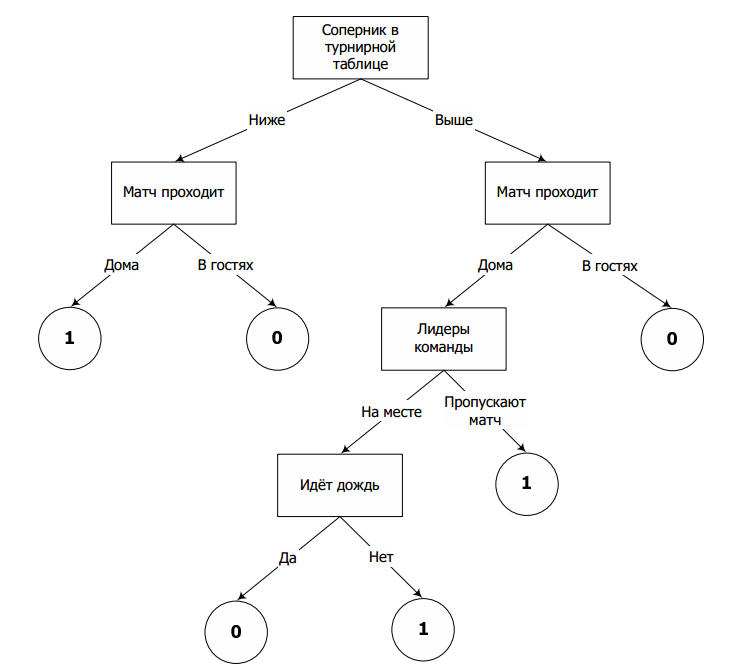
\includegraphics[height=190pt, keepaspectratio = true]{images/dtree}   
\end{figure}
\end{frame}

\begin{frame}\frametitle{Информативность}
	\begin{itemize}
		\item[--] Максимизировать количество правильно распознанных объектов класса $c$\\
		${ p_c(R) = \# \left\{ x_i: R(x_i) = 1 , y_i = c \right\} \rightarrow \max }$\\

		\item[--] Минимизировать количество объектов, ошибочно классифицированных как класс $c$\\
		${ n_c(R) = \# \left\{ x_i: R(x_i) = 1 , y_i \neq c \right\} \rightarrow \min }$\\
		
	\end{itemize}
\end{frame}

\begin{frame}\frametitle{Информативность}
\begin{figure}[htbp]
  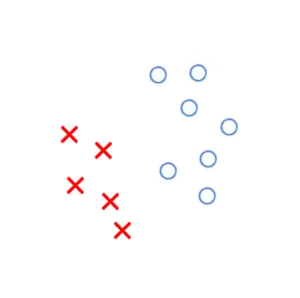
\includegraphics[height=190pt, keepaspectratio = true]{images/dtree_1}   
\end{figure}
\end{frame}

\begin{frame}\frametitle{Информативность}
\begin{figure}[htbp]
  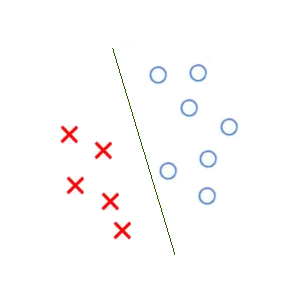
\includegraphics[height=190pt, keepaspectratio = true]{images/dtree_2}   
\end{figure}
\end{frame}

\begin{frame}\frametitle{Информативность}
\begin{figure}[htbp]
  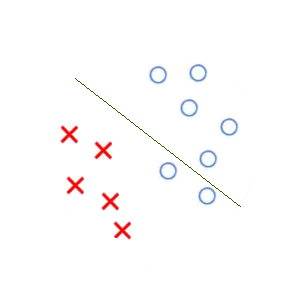
\includegraphics[height=190pt, keepaspectratio = true]{images/dtree_3}   
\end{figure}
\end{frame}

\begin{frame}\frametitle{Информативность}
\begin{figure}[htbp]
  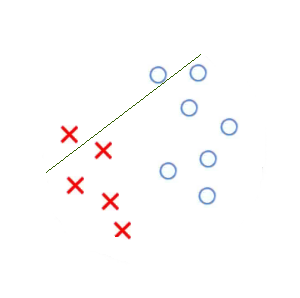
\includegraphics[height=190pt, keepaspectratio = true]{images/dtree_4}   
\end{figure}
\end{frame}

\begin{frame}\frametitle{Поиск закономерности}
\begin{figure}[htbp]
  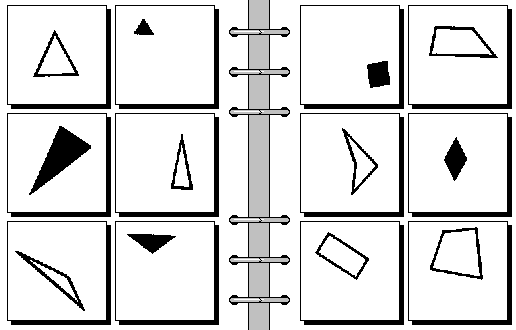
\includegraphics[height=150pt, keepaspectratio = true]{images/bongard6}   
\end{figure}
\end{frame}

\begin{frame}\frametitle{Поиск закономерности}
\begin{figure}[htbp]
  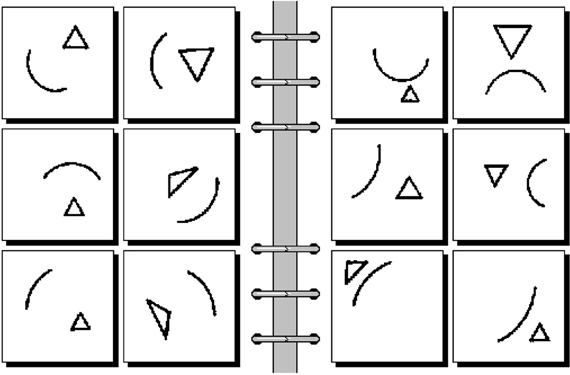
\includegraphics[height=150pt, keepaspectratio = true]{images/bongard40}   
\end{figure}
\end{frame}

\begin{frame}\frametitle{Поиск закономерности}
\begin{figure}[htbp]
  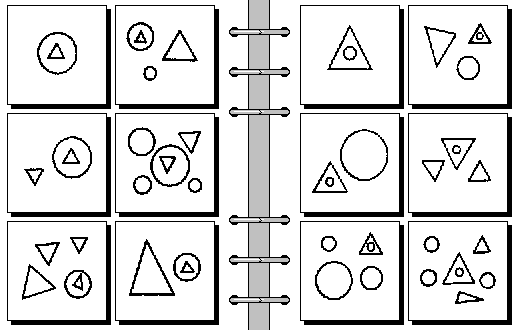
\includegraphics[height=150pt, keepaspectratio = true]{images/bongard47}   
\end{figure}
\end{frame}

\begin{frame}\frametitle{Поиск закономерности}
\begin{figure}[htbp]
  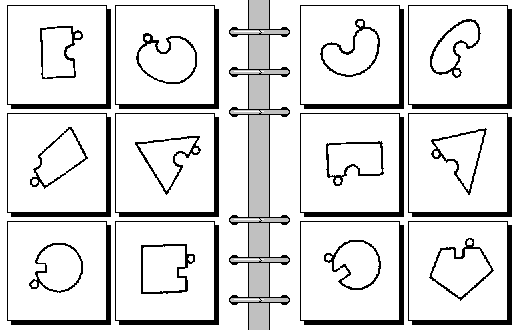
\includegraphics[height=150pt, keepaspectratio = true]{images/bongard55}   
\end{figure}
\end{frame}

\begin{frame}\frametitle{Основные вопросы}
	\begin{itemize}
		\item[--] Как изобретать признаки? 
		\item[--] Какого вида закономерности $R(x)$ нужны?
		\item[--] Как определять информативность? 
		\item[--] Как искать закономерности?
		\item[--] Как объединять закономерности в алгоритм?
	\end{itemize}
\end{frame}

\begin{frame}\frametitle{Виды правил}
\end{frame}

\begin{frame}\frametitle{Виды правил}
\begin{itemize}
\item[--] Пороговое условие (decision stump)
$R(x) = \left[f_j(x) \leq a_j \right]$ или  $\left[a_j \leq f_j(x) \leq b_j \right]$
\item[--] Конъюнкция $J$ пороговых условий
$R(x) = \bigwedge\limits_{j \in J} \left[a_j \leq f_j(x) \leq b_j \right]$
\item[--] Синдром -- выполнение не менее $d$ условий из $J$
$R(x) = \left[\sum\limits_{j \in J} \left[a_j \leq f_j(x) \leq b_j \right] \geq d \right]$
\end{itemize}
\end{frame}

\begin{frame}\frametitle{Оценивание информативности}
Идея: Хотим получить один критерий из двух:\\
\vspace{5mm}
${ p(R) = \# \left\{ x_i: R(x_i) = 1 , y_i = c \right\} \rightarrow \max  }$ 
${ n(R) = \# \left\{ x_i: R(x_i) = 1 , y_i \neq c \right\} \rightarrow \min}$ \\
\vspace{5mm}
	Очевидные свертки:\\
	\begin{itemize}
		\item[--] $I(p, n) = \frac{p}{p+n} \rightarrow \max$
		\item[--] $I(p, n) = p-n \rightarrow \max$
		\item[--] $I(p, n) = p-Cn \rightarrow \max$			
	\end{itemize}
\end{frame}

\begin{frame}\frametitle{Пример свертки двух критериев}
Пусть число примеров искомого класса P = 200 и число остальных объектов N=100\\
\vspace{5mm}
\begin{tabular}{|r l|l|l|l|}
  \hline 
  $p$ & $n$ & $p-n$ & $p-5n$ & $\frac{p}{p+n}$\\ 
  \hline \hline
  50 & 0 & \textcolor{red}{50} & 50 & 1\\
  \hline
  100 & 50 & \textcolor{red}{50} & -150 & 0.6\\
  \hline \hline
  50 & 9 & 41 & \textcolor{red}{5} & \textcolor{red}{0.84}\\
  \hline  
  5 & 0 & 5 & \textcolor{red}{5} & \textcolor{red}{1}\\  
  \hline 
\end{tabular}
\end{frame}

\begin{frame}\frametitle{Используемые критерии информативности}
\begin{enumerate}[--]
\item Information gain
$IGain(p,n) = h(\frac{P}{l}) - \frac{p+n}{l}h(\frac{p}{p+n}) - \frac{l-p-n}{l}h(\frac{P-p}{l-p-n}) \rightarrow \max$\\
где $h(q) = -q\log_2q - (1-q)\log_2(1-q)$
\item Gini impurity\\
$IGini(p,n)=IGain(p,n)$, где $h(q)=4q(1-q)$
\item Fisher’s Exact Test\\
$IStat(p,n) = -\frac{1}{l}\log_2\frac{C_P^pC_N^n}{C_{P+N}^{p+n}} \rightarrow \max$
\item Boosting\\
$\sqrt{p} - \sqrt{n} \rightarrow \max$
\end{enumerate}

\end{frame}

%\begin{frame}\frametitle{Закономерности в pn области}
%\textcolor{red}{TODO: картинка}
%\end{frame}



\begin{frame}\frametitle{Поиск информативных закономерностей}
Input: Обучающая выборка $X^l$\\
Output: Множество закономерностей $Z$\\
\vspace{5mm}
Выбрать начальное множество $Z$\\
Повторять пока правила улучшаются:\\
\hspace{10mm} $Z'=$ множество модификаций правил $R \in Z$\\
\hspace{10mm} Удалить слишком похожие правила из $Z \cup Z'$\\
\hspace{10mm} Оценить инфомативность правил $R \in Z'$\\
\hspace{10mm} $Z=$ наиболее информативные правила из $Z \cup Z'$\\
\vspace{5mm}
Примеры:\\
\begin{enumerate}[--]
	\item Генетические алгоритмы
	\item Метод ветвей и границ	
	\item Стохастический локальный поиск	
\end{enumerate}

\end{frame}

\begin{frame}\frametitle{Критерий Парето}
Парето-фронт -- множество недоминируемых закономерностей (правее и ниже точек нет)
\begin{figure}[htbp]
  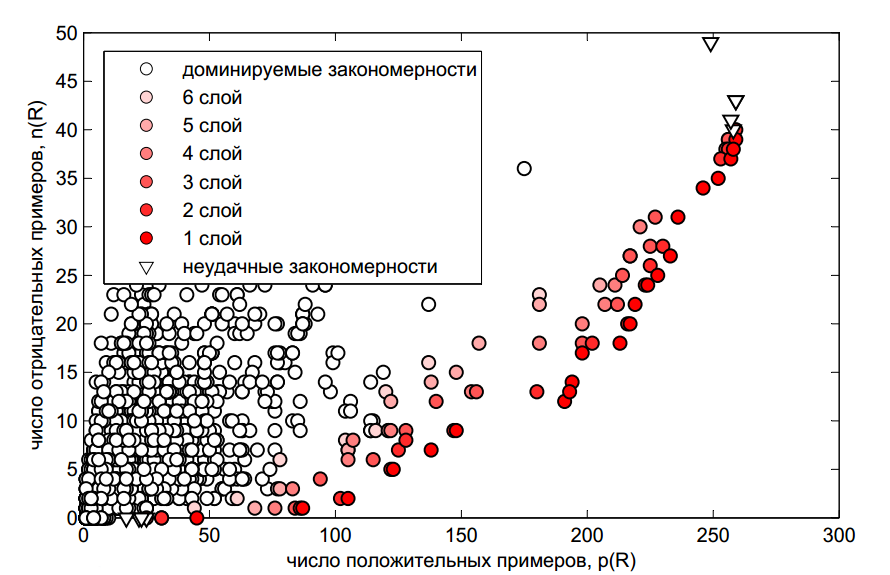
\includegraphics[height=150pt, keepaspectratio = true]{images/pareto}   
\end{figure}
\footnotesize\textcolor{gray} {Картинка с machinelearning.ru}
\end{frame}

\begin{frame}\frametitle{Вопрос}
Как собрать классификатор из закономерностей?
\end{frame}

\begin{frame}\frametitle{Решающий список}
Множество классов $c_1,c_2,\dots, c_T \in Y$\\
\vspace{5mm}
Идея:\\
Возьмем $R_1(x), R_2(x), \dots, R_T(x)$ закономерностей и будем по порядку применять на объекте. 
Как только предикат $R_i$ сработал -- вернем соответствующий класс $c_i$.
\end{frame}

\begin{frame}\frametitle{Решающий список}
Множество классов $c_1,c_2,\dots, c_T \in Y$\\
\vspace{5mm}
Идея:\\
Возьмем $R_1(x), R_2(x), \dots, R_T(x)$ закономерностей и будем по порядку применять на объекте. 
Как только предикат $R_i$ сработал -- вернем соответствующий класс $c_i$.\\
\vspace{5mm}
$E(R_i, X^l) = \frac{n(R_i)}{n(R_i)+p(R_i)} \rightarrow \min$ -- доля ошибок $R_i$ на $X^l$\\
Т.к. каждое правило принимает окончательное решение $\Rightarrow$ ошибка правила равна ошибке всего алгоритма
\end{frame}

\begin{frame}\frametitle{Жадный алгоритм для решающего списка}
Input: $X^l$, семейство предикатов $\mathcal{B}$, $T_{max}$, $I_{min}$, $E_{max}$, $l_0$\\
Output: Решающий список $\left\{ R_i, c_i \right\}_{i=1}^T$\\
\vspace{5mm}
$U = X^l$\\
Для всех $i = 1,2,\dots,T_{max}$\\
\hspace{10mm} Выбрать класс $c_i$\\
\hspace{10mm} Максимизировать информативность при \\
\hspace{40mm} ограничении на число ошибок\\
\hspace{10mm} Если $I(R_i, U) < I_{min}$ выйти\\
\hspace{10mm} Убрать объекты, покрытые правилом $R_i$\\
\hspace{10mm} Если $\vert U \vert \leq l_0$ выйти
\end{frame}

\begin{frame}\frametitle{Жадный алгоритм для решающего списка}
Input: $X^l$, семейство предикатов $\mathcal{B}$, $T_{max}$, $I_{min}$, $E_{max}$, $l_0$\\
Output: Решающий список $\left\{ R_i, c_i \right\}_{i=1}^T$\\
\vspace{5mm}
$U = X^l$\\
Для всех $i = 1,2,\dots,T_{max}$\\
\hspace{10mm} Выбрать класс $c_i$\\
\hspace{10mm} $R_i = \max\limits_{E(R, U) \leq E_{max}} I(R, U)$\\
\hspace{10mm} Если $I(R_i, U) < I_{min}$ выйти\\
\hspace{10mm} $U = \left\{ x \in U: R_i(x) = 0 \right\}$\\
\hspace{10mm} Если $\vert U \vert \leq l_0$ выйти
\end{frame}

\begin{frame}\frametitle{Наблюдения}
\begin{enumerate}[--]
\item Низкое качество классификации
\item Разные стратегии выбора класса $c_i$
\item Подбор параметра $E_{max}$
\end{enumerate}
\end{frame}

\begin{frame}\frametitle{Наблюдения}
\begin{enumerate}[--]
\item Низкое качество классификации
\item Разные стратегии выбора класса $c_i$
\item Подбор параметра $E_{max}$
\end{enumerate}
\vspace{5mm}
Параметр $E_{max}$ влияет на сложность списка:\\
$E_{max} \downarrow$ $\Rightarrow$ $p(R_i) \downarrow, T \uparrow$
\end{frame}

\begin{frame}\frametitle{Бинарное решающее дерево}
Бинарное решающее дерево -- алгоритм классификации a(x), задающийся бинарным деревом:\\
\begin{enumerate}[--]
\item $\forall v \in V_{in} \rightarrow \beta_v: X \rightarrow \left\{ 0,1\right\}$, $\beta \in \mathcal{B}$
\item $\forall v \in V_{leaf} \rightarrow $ имя класса $c_v \in Y$\\

\begin{figure}[htbp]
  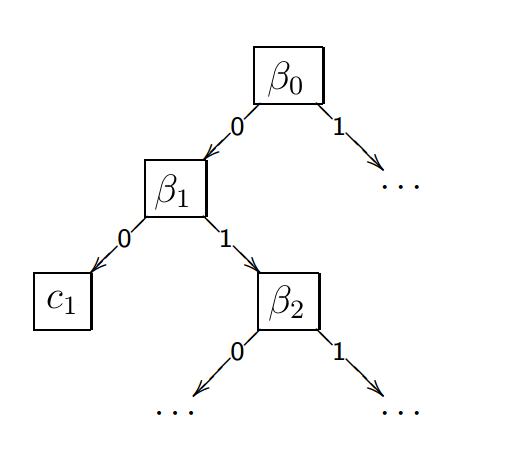
\includegraphics[height=150pt, keepaspectratio = true]{images/binary_tree}   
\end{figure}
\end{enumerate}
\end{frame}

\begin{frame}\frametitle{Пример решающего дерева}
\textcolor{red}{TODO}
\end{frame}

\begin{frame}\frametitle{Алгоритм построения ID3}
\textcolor{red}{TODO}
\end{frame}

\begin{frame}\frametitle{Плюсы и минусы}
\begin{enumerate}[+]
\item Интерпретируемость и простота классификации
\item Допустимы разнотипные данные и данные с пропусками
\item Не бывает отказов от классификации
\item Трудоёмкость линейна по длине выборки
\end{enumerate}
\begin{enumerate}[-]
\item Жадный ID3 сильно переобучается
\item Высокая чувствительность к шуму, к составу выборки, к критерию информативности
\item 
\end{enumerate}
\end{frame}

\begin{frame}\frametitle{Усечение дерева C4.5}
\textcolor{red}{TODO}
\end{frame}

\begin{frame}\frametitle{ODT}
\textcolor{red}{TODO}
\end{frame}

\begin{frame}\frametitle{Random forest}
\textcolor{red}{TODO}
\end{frame}

\begin{frame}\frametitle{На следующей лекции}
\begin{itemize}
\item[--] Байесовские методы классификации
\end{itemize}
\end{frame}
\end{document}
